\chapter{Järjestäminen}

\emph{Järjestäminen} on keskeinen algoritmiikan ongelma,
jossa meillä on $n$ alkiota sisältävä aineisto
ja haluamme järjestää sen suuruusjärjestykseen.
Esimerkiksi jos meillä on taulukko $[5,2,4,2,6,1]$ ja
järjestämme alkiot pienimmästä suurimpaan,
tuloksena on taulukko $[1,2,2,4,5,6]$.

Tavoitteemme on toteuttaa järjestäminen
\emph{tehokkaasti}.
On helppoa toteuttaa järjestäminen ajassa $O(n^2)$,
mutta tämä on liian hidasta suurella aineistolla.
Tässä luvussa opimme kaksi tehokasta
järjestämisalgoritmia, jotka vievät aikaa vain $O(n \log n)$.
Toisaalta osoittautuu, että ei ole olemassa
yleistä järjestämisalgoritmia, joka toimisi nopeammin
kuin $O(n \log n)$.

Voimme käyttää järjestämistä monella tavalla
algoritmien suunnittelussa.
Usein voimme helpottaa ongelman ratkaisemista
järjestämällä ensin aineiston.
Esimerkiksi jos haluamme tutkia,
mikä alkio esiintyy useimmiten taulukossa,
voimme järjestää ensin taulukon sisällön,
jolloin yhtä suuret alkiot päätyvät vierekkäin.
Tämän jälkeen meidän riittää käydä taulukko läpi
ja etsiä siitä pisin samaa alkiota toistava osuus.

\section{Järjestäminen ajassa $O(n^2)$}

Tutustumme aluksi yksinkertaiseen järjestämisalgoritmiin
nimeltä lisäysjär\-jestäminen,
joka järjestää $n$-alkioisen aineiston ajassa $O(n^2)$.
Vaikka algoritmi ei ole nopea, se on tutustumisen arvoinen
ja antaa hyvän lähtökohdan tehokkaampien algoritmien
suunnittelemiselle.

\subsection{Lisäysjärjestäminen}

\emph{Lisäysjärjestäminen} käy läpi taulukon
vasemmalta oikealle.
Kun algoritmi tulee tiettyyn taulukon kohtaan,
se siirtää kyseisessä kohdassa olevan alkion
oikeaan paikkaan taulukon
alkuosassa niin, että taulukon alkuosa
on tämän jälkeen järjestyksessä.
Niinpä kun algoritmi pääsee taulukon loppuun,
koko taulukko on järjestyksessä.

\begin{figure}
\center
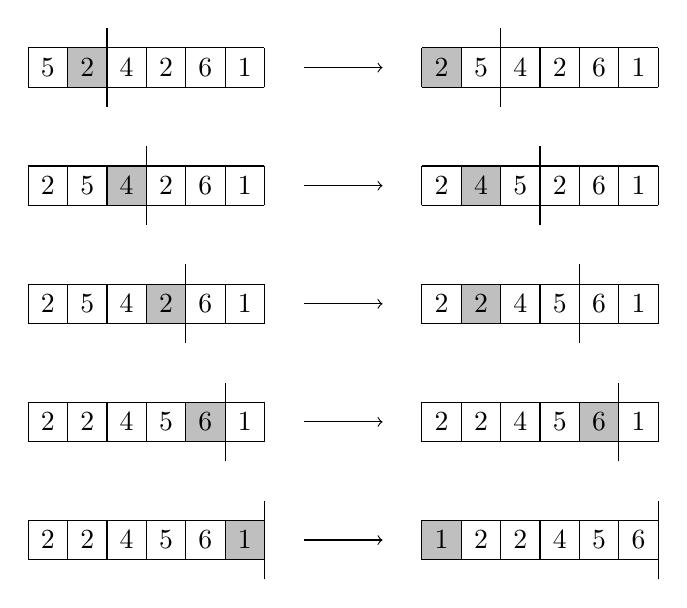
\begin{tikzpicture}[scale=0.5]
\begin{scope}
\fill[lightgray] (1,0) rectangle (2,1);
\draw (0,0) grid (6,1);
\foreach \x/\v in {0/5,1/2,2/4,3/2,4/6,5/1} \node at (0.5+\x,0.5) {\v};
\draw (2,-0.5) -- (2,1.5);
\draw[->] (7,0.5) -- (9,0.5);
\end{scope}
\begin{scope}[xshift=10cm]
\fill[lightgray] (0,0) rectangle (1,1);
\draw (0,0) grid (6,1);
\foreach \x/\v in {0/2,1/5,2/4,3/2,4/6,5/1} \node at (0.5+\x,0.5) {\v};
\draw (2,-0.5) -- (2,1.5);
\end{scope}
\begin{scope}[yshift=-3cm]
\fill[lightgray] (2,0) rectangle (3,1);
\draw (0,0) grid (6,1);
\foreach \x/\v in {0/2,1/5,2/4,3/2,4/6,5/1} \node at (0.5+\x,0.5) {\v};
\draw (3,-0.5) -- (3,1.5);
\draw[->] (7,0.5) -- (9,0.5);
\end{scope}
\begin{scope}[yshift=-3cm,xshift=10cm]
\fill[lightgray] (1,0) rectangle (2,1);
\draw (0,0) grid (6,1);
\foreach \x/\v in {0/2,1/4,2/5,3/2,4/6,5/1} \node at (0.5+\x,0.5) {\v};
\draw (3,-0.5) -- (3,1.5);
\end{scope}
\begin{scope}[yshift=-6cm]
\fill[lightgray] (3,0) rectangle (4,1);
\draw (0,0) grid (6,1);
\foreach \x/\v in {0/2,1/5,2/4,3/2,4/6,5/1} \node at (0.5+\x,0.5) {\v};
\draw (4,-0.5) -- (4,1.5);
\draw[->] (7,0.5) -- (9,0.5);
\end{scope}
\begin{scope}[yshift=-6cm,xshift=10cm]
\fill[lightgray] (1,0) rectangle (2,1);
\draw (0,0) grid (6,1);
\foreach \x/\v in {0/2,1/2,2/4,3/5,4/6,5/1} \node at (0.5+\x,0.5) {\v};
\draw (4,-0.5) -- (4,1.5);
\end{scope}
\begin{scope}[yshift=-9cm]
\fill[lightgray] (4,0) rectangle (5,1);
\draw (0,0) grid (6,1);
\foreach \x/\v in {0/2,1/2,2/4,3/5,4/6,5/1} \node at (0.5+\x,0.5) {\v};
\draw (5,-0.5) -- (5,1.5);
\draw[->] (7,0.5) -- (9,0.5);
\end{scope}
\begin{scope}[yshift=-9cm,xshift=10cm]
\fill[lightgray] (4,0) rectangle (5,1);
\draw (0,0) grid (6,1);
\foreach \x/\v in {0/2,1/2,2/4,3/5,4/6,5/1} \node at (0.5+\x,0.5) {\v};
\draw (5,-0.5) -- (5,1.5);
\end{scope}
\begin{scope}[yshift=-12cm]
\fill[lightgray] (5,0) rectangle (6,1);
\draw (0,0) grid (6,1);
\foreach \x/\v in {0/2,1/2,2/4,3/5,4/6,5/1} \node at (0.5+\x,0.5) {\v};
\draw (6,-0.5) -- (6,1.5);
\draw[->] (7,0.5) -- (9,0.5);
\end{scope}
\begin{scope}[yshift=-12cm,xshift=10cm]
\fill[lightgray] (0,0) rectangle (1,1);
\draw (0,0) grid (6,1);
\foreach \x/\v in {0/1,1/2,2/2,3/4,4/5,5/6} \node at (0.5+\x,0.5) {\v};
\draw (6,-0.5) -- (6,1.5);
\end{scope}
\end{tikzpicture}
\caption{Lisäysjärjestäminen taulukolle $[5,2,4,2,6,1]$.}
\label{fig:lisjar}
\end{figure}

Kuva \ref{fig:lisjar} näyttää esimerkin lisäysjärjestämisen
toiminnasta, kun järjes\-tämme taulukon $[5,2,4,2,6,1]$.
Jokaisella rivillä siirrämme harmaataustaisen alkion
sen oikealle paikalle taulukon alkuosassa.
Pystyviiva ilmaisee kohdan, johon asti taulukko on järjestyksessä
siirron jälkeen.
Lopulta saamme aikaan järjestetyn taulukon $[1,2,2,4,5,6]$.

Seuraava koodi toteuttaa lisäysjärjestämisen:

\begin{code}
for i = 1 to n-1
    j = i-1
    while j >= 0 and taulu[j] > taulu[j+1]:
        swap(taulu[j],taulu[j+1])
        j--
\end{code}

Jokaisen indeksin $i$ kohdalla siirrämme taulukon
kohdassa $i$ olevan alkion sen oikealle paikalle
taulukon alkuosassa.
Teemme tämän vaihtamalla joka askeleella keskenään
alkion ja sen vasemmalla puolella olevan alkion
niin kauan, kunnes alkio on oikealla paikalla.

Lisäysjärjestämisen tehokkuus riippuu siitä,
mikä on järjestettävän taulukon sisältö.
Algoritmi toimii sitä paremmin, mitä lähempänä järjestystä
taulukko on valmiiksi.
Jos taulukko on järjestyksessä,
aikaa kuluu vain $\Theta(n)$, koska meidän ei tarvitse siirtää
mitään alkioita.
Pahin tapaus algoritmille on kuitenkin, että taulukko on
\emph{käänteisessä} järjestyksessä,
jolloin joudumme siirtämään jokaisen alkion
taulukon alkuun ja aikaa kuluu $\Theta(n^2)$.

\subsection{Inversiot}

Hyödyllinen käsite järjestämisalgoritmien analysoinnissa
on \emph{inversio}: kaksi taulukossa olevaa alkiota,
jotka ovat väärässä järjestyksessä.
Esimerkiksi taulukossa $[3,1,4,2]$ on kolme inversiota:
$(3,1)$, $(3,2)$ ja $(4,2)$.
Inversioiden määrä kertoo meille taulukon järjestyksestä:
mitä vähemmän inversioita taulukossa on,
sitä lähempänä se on järjestystä.
Erityisesti taulukko on järjestyksessä tarkalleen silloin,
kun siinä ei ole yhtään inversiota.

Kun järjestämisalgoritmi järjestää taulukon,
se \emph{poistaa} siitä inversioita.
Aina kun lisäysjärjestäminen vaihtaa kaksi
väärin päin olevaa alkiota keskenään,
se poistaa taulukosta yhden inversion.
Niinpä lisäysjärjestämisen työmäärä on yhtä suuri
kuin järjestettävän taulukon inversioiden määrä.

Olemme jo todenneet, että pahin mahdollinen syöte
lisäysjärjestämiselle on käänteisessä järjestyksessä oleva taulukko.
Tällaisessa taulukossa jokainen alkiopari muodostaa inversion,
joten inversioiden määrä on
\[1+2+\dots+(n-1)=\frac{n(n-1)}{2}=\Theta(n^2).\]
Entä kuinka hyvin algoritmi toimii \emph{keskimäärin}?
Jos oletamme, että taulukossa on $n$ eri alkiota satunnaisessa
järjestyksessä, alkiopari muodostaa inversion todennäköisyydellä $1/2$.
Niinpä inversioiden määrän \emph{odotusarvo} on
\[\frac{n(n-1)}{4}=\Theta(n^2),\]
eli aikaa kuluu neliöllinen määrä myös keskimääräisessä
tapauksessa.

Syy lisäysjärjestämisen hitauteen on siis,
että se ei poista taulukosta inversioita riittävän tehokkaasti.
Jos haluamme kehittää paremman järjestämis\-algoritmin,
meidän täytyy suunnitella se niin, että se voi poistaa
useita inversiota \emph{yhtä aikaa}.
Käytännössä algoritmin täytyy pystyä siirtämään
väärässä paikassa oleva alkio tehokkaasti taulukon
toiselle puolelle.

\section{Järjestäminen ajassa $O(n \log n)$}

Seuraavaksi tutustumme kahteen tehokkaaseen
järjestämisalgoritmiin, jotka perustuvat
\emph{hajota ja hallitse} -tekniikkaan.
Ideana on, että kun saamme järjestettäväksi taulukon,
jaamme ongelman rekursiivisesti pienemmiksi osa\-ongelmiksi,
joissa meidän riittää järjestää pienempiä taulukoita.

\subsection{Lomitusjärjestäminen}

\begin{figure}
\center
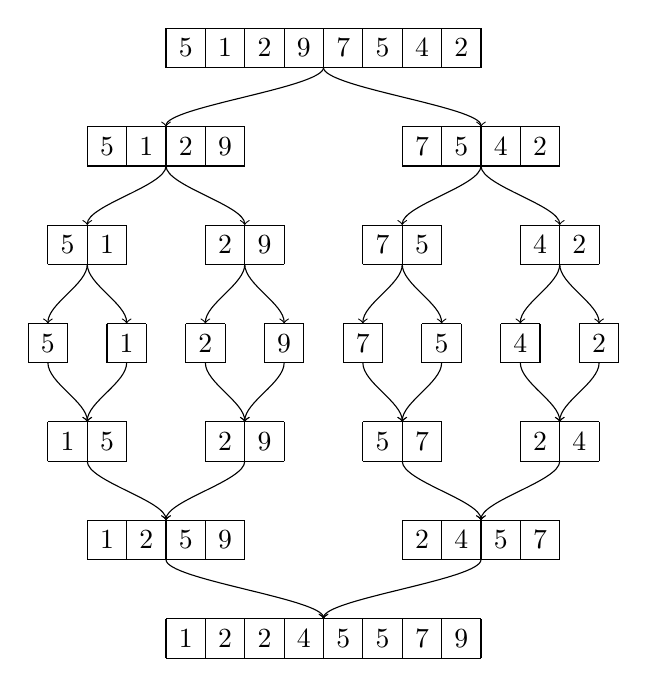
\begin{tikzpicture}[scale=0.5]
\begin{scope}
\draw (0,0) grid (8,1);
\foreach \x/\v in {0/5,1/1,2/2,3/9,4/7,5/5,6/4,7/2} \node at (0.5+\x,0.5) {\v};
\draw[->] (4,0) .. controls (4,-0.5) and (0,-1) .. (0,-1.5);
\draw[->] (4,0) .. controls (4,-0.5) and (8,-1) .. (8,-1.5);
\end{scope}
\begin{scope}[yshift=-2.5cm,xshift=-2cm]
\draw (0,0) grid (4,1);
\draw (8,0) grid (12,1);
\foreach \x/\v in {0/5,1/1,2/2,3/9,8/7,9/5,10/4,11/2} \node at (0.5+\x,0.5) {\v};
\draw[->] (2,0) .. controls (2,-0.5) and (0,-1) .. (0,-1.5);
\draw[->] (2,0) .. controls (2,-0.5) and (4,-1) .. (4,-1.5);
\draw[->] (10,0) .. controls (10,-0.5) and (8,-1) .. (8,-1.5);
\draw[->] (10,0) .. controls (10,-0.5) and (12,-1) .. (12,-1.5);
\end{scope}
\begin{scope}[yshift=-5cm,xshift=-3cm]
\draw (0,0) grid (2,1);
\draw (4,0) grid (6,1);
\draw (8,0) grid (10,1);
\draw (12,0) grid (14,1);
\foreach \x/\v in {0/5,1/1,4/2,5/9,8/7,9/5,12/4,13/2} \node at (0.5+\x,0.5) {\v};
\draw[->] (1,0) .. controls (1,-0.5) and (0,-1) .. (0,-1.5);
\draw[->] (1,0) .. controls (1,-0.5) and (2,-1) .. (2,-1.5);
\draw[->] (5,0) .. controls (5,-0.5) and (4,-1) .. (4,-1.5);
\draw[->] (5,0) .. controls (5,-0.5) and (6,-1) .. (6,-1.5);
\draw[->] (9,0) .. controls (9,-0.5) and (8,-1) .. (8,-1.5);
\draw[->] (9,0) .. controls (9,-0.5) and (10,-1) .. (10,-1.5);
\draw[->] (13,0) .. controls (13,-0.5) and (12,-1) .. (12,-1.5);
\draw[->] (13,0) .. controls (13,-0.5) and (14,-1) .. (14,-1.5);
\end{scope}
\begin{scope}[yshift=-7.5cm,xshift=-3.5cm]
\draw (0,0) grid (1,1);
\draw (2,0) grid (3,1);
\draw (4,0) grid (5,1);
\draw (6,0) grid (7,1);
\draw (8,0) grid (9,1);
\draw (10,0) grid (11,1);
\draw (12,0) grid (13,1);
\draw (14,0) grid (15,1);
\foreach \x/\v in {0/5,2/1,4/2,6/9,8/7,10/5,12/4,14/2} \node at (0.5+\x,0.5) {\v};
\draw[->] (0.5,0) .. controls (0.5,-0.5) and (1.5,-1) .. (1.5,-1.5);
\draw[->] (2.5,0) .. controls (2.5,-0.5) and (1.5,-1) .. (1.5,-1.5);
\draw[->] (4.5,0) .. controls (4.5,-0.5) and (5.5,-1) .. (5.5,-1.5);
\draw[->] (6.5,0) .. controls (6.5,-0.5) and (5.5,-1) .. (5.5,-1.5);
\draw[->] (8.5,0) .. controls (8.5,-0.5) and (9.5,-1) .. (9.5,-1.5);
\draw[->] (10.5,0) .. controls (10.5,-0.5) and (9.5,-1) .. (9.5,-1.5);
\draw[->] (12.5,0) .. controls (12.5,-0.5) and (13.5,-1) .. (13.5,-1.5);
\draw[->] (14.5,0) .. controls (14.5,-0.5) and (13.5,-1) .. (13.5,-1.5);
\end{scope}
\begin{scope}[yshift=-10cm,xshift=-3cm]
\draw (0,0) grid (2,1);
\draw (4,0) grid (6,1);
\draw (8,0) grid (10,1);
\draw (12,0) grid (14,1);
\foreach \x/\v in {0/1,1/5,4/2,5/9,8/5,9/7,12/2,13/4} \node at (0.5+\x,0.5) {\v};
\draw[->] (1,0) .. controls (1,-0.5) and (3,-1) .. (3,-1.5);
\draw[->] (5,0) .. controls (5,-0.5) and (3,-1) .. (3,-1.5);
\draw[->] (9,0) .. controls (9,-0.5) and (11,-1) .. (11,-1.5);
\draw[->] (13,0) .. controls (13,-0.5) and (11,-1) .. (11,-1.5);
\end{scope}
\begin{scope}[yshift=-12.5cm,xshift=-2cm]
\draw (0,0) grid (4,1);
\draw (8,0) grid (12,1);
\foreach \x/\v in {0/1,1/2,2/5,3/9,8/2,9/4,10/5,11/7} \node at (0.5+\x,0.5) {\v};
\draw[->] (2,0) .. controls (2,-0.5) and (6,-1) .. (6,-1.5);
\draw[->] (10,0) .. controls (10,-0.5) and (6,-1) .. (6,-1.5);
\end{scope}
\begin{scope}[yshift=-15cm]
\draw (0,0) grid (8,1);
\foreach \x/\v in {0/1,1/2,2/2,3/4,4/5,5/5,6/7,7/9} \node at (0.5+\x,0.5) {\v};
\end{scope}
\end{tikzpicture}
\caption{Lomitusjärjestäminen taulukolle $[5,1,2,9,7,5,4,2]$.}
\label{fig:lomjar}
\end{figure}

\emph{Lomitusjärjestäminen} on rekursiivinen järjestämisalgoritmi,
joka perustuu taulukon puolituksiin.
Kun saamme järjestettäväksi $n$-kokoisen taulukon,
jaamme sen keskeltä kahdeksi osataulukoksi,
joissa molemmissa on noin $n/2$ alkiota.
Tämän jälkeen järjestämme molemmat osataulukot erikseen rekursiivisesti.
Lopuksi \emph{lomitamme} järjestetyt osataulukot niin,
että niistä muodostuu kokonainen järjestetty taulukko.
Pohjatapauksena jos $n=1$,
taulukko on valmiiksi järjestyksessä eikä
meidän tarvitse tehdä mitään.

Seuraava koodi esittää tarkemmin lomitusjärjestämisen toiminnan:

\begin{code}
jarjesta(a,b)
    if a == b
        return
    k = (a+b)/2
    jarjesta(a,k-1)
    jarjesta(k,b)
    lomita(a,k-1,k,b)
\end{code}

Algoritmi järjestää taulukon osataulukon kohdasta
$a$ kohtaan $b$, eli kun haluamme järjestää koko taulukon,
kutsumme algoritmia parametreilla $a=0$ ja $b=n-1$.
Tarkastamme ensin, onko osataulukossa vain yksi alkio,
ja jos on, poistumme algoritmista.
Sitten laskemme muuttujaan $k$ järjestettävän välin keskikohdan
ja järjestämme vasemman ja oikean puoliskon rekursiivisesti.
Lopuksi kutsumme algoritmia \texttt{lomita},
joka muodostaa kokonaisen järjestetyn taulukon osataulukoista.

Kuva \ref{fig:lomjar} näyttää, miten lomitusjärjestäminen
toimii, kun sille annetaan taulukko $[5,1,2,9,7,5,4,2]$.
Algoritmi puolittaa ensin taulukon kahdeksi osataulukoksi
$[5,1,2,9]$ ja $[7,5,4,2]$ ja järjestää molemmat
osataulukot kutsumalla itseään.
Seuraavaksi järjestettävänä on osataulukko $[5,1,2,9]$,
jonka algoritmi jakaa osataulukoiksi $[5,1]$ ja $[2,9]$, jne.
Lopulta jäljellä on vain yhden alkion kokoisia
osataulukoita, jotka ovat valmiiksi järjestyksessä.
Tällöin rekursiivinen jakautuminen päättyy ja algoritmi
alkaa koota järjestettyjä osataulukkoja pienimmästä suurimpaan.

Oleellinen seikka algoritmin tehokkuuden kannalta on,
miten nopeasti pystymme lomittamaan järjestetyt osataulukot.
Tämä on mahdollista lineaarisessa ajassa käyttäen hyväksi tietoa,
että osataulukot ovat järjestyksessä.
Tämän ansiosta voimme käydä osataulukoita rinnakkain läpi
vasemmalta oikealle ja valita aina seuraavaksi pienimmän alkion
kahdesta vaihtoehdosta lopulliseen järjestettyyn taulukkoon.

Nyt voimme määrittää, kuinka tehokas lomitusjärjestäminen on.
Rekursion ylimmällä tasolla taulukon koko on $n$,
seuraavalla tasolla $n/2$, tämän jälkeen $n/4$, jne.,
joten tasoja on yhteensä $O(\log n)$, ennen kuin pääsemme
osataulukoihin, joissa on vain yksi alkio.
Jokaisen tason käsitteleminen vie yhteensä aikaa $O(n)$,
koska lomittaminen on lineaarista.
Niinpä algoritmin kokonaisaikavaativuus on $O(n \log n)$.

\subsection{Pikajärjestäminen}

\emph{Pikajärjestäminen} tarjoaa toisenlaisen rekursiivisen
lähestymistavan taulukon järjestämiseen.
Kun saamme järjestettäväksi taulukon, valitsemme ensin jonkin
sen alkioista \emph{jakoalkioksi}.
Tämän jälkeen siirrämme alkioita niin,
että jakoalkion vasemmalle puolelle tulevat kaikki sitä pienemmät alkiot
ja oikealle puolelle tulevat kaikki muut alkiot.
Lopuksi järjestämme rekursiivisesti vasemman ja oikean puolen alkiot.

Seuraava koodi esittää pikajärjestämisen toiminnan:

\begin{code}
jarjesta(int a, int b)
    if (a >= b)
        return
    k = jako(a,b)
    jarjesta(a,k-1)
    jarjesta(k+1,b)
\end{code}

Algoritmille annetaan parametrina järjestettävä
taulukon osataulukko.
Jos osataulukko on tyhjä tai siinä on vain yksi alkio,
poistumme algoritmista.
Muuten kutsumme algoritmia \texttt{jako}, joka valitsee jakoalkion,
siirtää muut alkiot sen vasemmalle ja oikealle puolelle
ja palauttaa sitten taulukon kohdan, jossa jakoalkio on siirtojen jälkeen.
Sitten kutsumme algoritmia rekursiivisesti
taulukon vasempaan ja oikeaan osaan.


\begin{figure}
\center
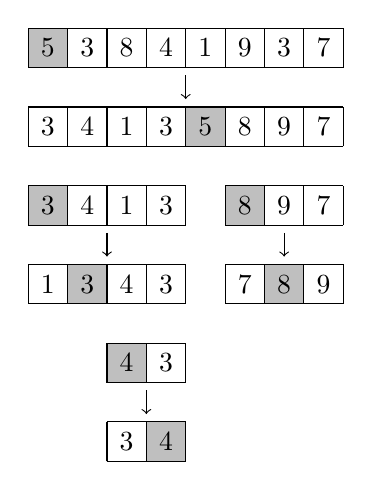
\begin{tikzpicture}[scale=0.5]
\begin{scope}
\fill[color=lightgray] (0,0) rectangle (1,1);
\draw (0,0) grid (8,1);
\foreach \x/\v in {0/5,1/3,2/8,3/4,4/1,5/9,6/3,7/7} \node at (0.5+\x,0.5) {\v};
\fill[color=lightgray] (4,-2) rectangle (5,-1);
\draw (0,-2) grid (8,-1);
\foreach \x/\v in {0/3,1/4,2/1,3/3,4/5,5/8,6/9,7/7} \node at (0.5+\x,-1.5) {\v};
\draw[->] (4,-0.2) -- (4,-0.8);
\end{scope}
\begin{scope}[xshift=0cm,yshift=-4cm]
\fill[color=lightgray] (0,0) rectangle (1,1);
\draw (0,0) grid (4,1);
\foreach \x/\v in {0/3,1/4,2/1,3/3} \node at (0.5+\x,0.5) {\v};
\fill[color=lightgray] (1,-2) rectangle (2,-1);
\draw (0,-2) grid (4,-1);
\foreach \x/\v in {0/1,1/3,2/4,3/3} \node at (0.5+\x,-1.5) {\v};
\draw[->] (2,-0.2) -- (2,-0.8);
\end{scope}
\begin{scope}[xshift=5cm,yshift=-4cm]
\fill[color=lightgray] (0,0) rectangle (1,1);
\draw (0,0) grid (3,1);
\foreach \x/\v in {0/8,1/9,2/7} \node at (0.5+\x,0.5) {\v};
\fill[color=lightgray] (1,-2) rectangle (2,-1);
\draw (0,-2) grid (3,-1);
\foreach \x/\v in {0/7,1/8,2/9} \node at (0.5+\x,-1.5) {\v};
\draw[->] (1.5,-0.2) -- (1.5,-0.8);
\end{scope}
\begin{scope}[xshift=2cm,yshift=-8cm]
\fill[color=lightgray] (0,0) rectangle (1,1);
\draw (0,0) grid (2,1);
\foreach \x/\v in {0/4,1/3} \node at (0.5+\x,0.5) {\v};
\fill[color=lightgray] (1,-2) rectangle (2,-1);
\draw (0,-2) grid (2,-1);
\foreach \x/\v in {0/3,1/4} \node at (0.5+\x,-1.5) {\v};
\draw[->] (1,-0.2) -- (1,-0.8);
\end{scope}
\end{tikzpicture}
\caption{Pikajärjestäminen taulukolle $[5,3,8,4,1,9,3,7]$.}
\label{fig:pikjar}
\end{figure}

Kuva \ref{fig:pikjar} näyttää, miten pikajärjestäminen toimii, kun sille
annetaan taulukko $[5,3,8,4,1,9,3,7]$.
Meidän täytyy ensin päättää jokin tapa,
miten valitsemme jakoalkion algoritmin aikana.
Toimimme tässä esimerkissä niin, että jakoalkio on aina
taulukon \emph{ensimmäinen} alkio.
Kun aloitamme järjestämisen, koko taulukon jakoalkio on 5
ja siirrämme sen vasemmalle puolelle
alkiot $[3,4,1,3]$ ja oikealle puolelle alkiot $[8,9,7]$.
Tämän jälkeen järjestämme vasemman ja oikean puolen rekursiivisesti vastaavasti.

Pikajärjestämisen tehokkuuteen vaikuttaa, miten valitsemme jakoalkion.
Haluaisimme valita jakoalkion niin, että sen vasemmalle ja oikealle
puolelle siirretään suunnilleen yhtä monta alkiota.
Jos onnistumme tässä, taulukon koko puolittuu jokaisen jaon jälkeen
ja pikajärjestäminen toimii tehokkaasti.
Koska pystymme siirtämään alkiot jakoalkion ympärille
lineaarisessa ajassa, pikajärjestäminen vie tässä tapauksessa aikaa
$O(n \log n)$ samaan tapaan kuin lomitusjärjestäminen.

Uhkana on kuitenkin, että valitsemme jakoalkion huonosti ja se jakaa
taulukon osiin epätasaisesti.
Kuva \ref{fig:pikpah} näyttää tilanteen, jossa jokaisessa jaossa
kaikki alkiot jäävät jakoalkion oikealle puolelle.
Tällöin pikajärjestäminen viekin aikaa $O(n^2)$, koska rekursiivisia
tasoja on $O(n)$.
Selvästikään \emph{ei} ole hyvä tapa valita taulukon ensimmäinen
alkio jakoalkioksi, koska silloin valmiiksi järjestyksessä olevan
taulukon järjestäminen vie aikaa $O(n^2)$.
\begin{figure}
\center
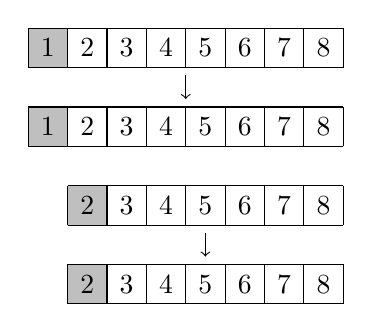
\begin{tikzpicture}[scale=0.5]
\begin{scope}
\fill[color=lightgray] (0,0) rectangle (1,1);
\draw (0,0) grid (8,1);
\foreach \x/\v in {0/1,1/2,2/3,3/4,4/5,5/6,6/7,7/8} \node at (0.5+\x,0.5) {\v};
\fill[color=lightgray] (0,-2) rectangle (1,-1);
\draw (0,-2) grid (8,-1);
\foreach \x/\v in {0/1,1/2,2/3,3/4,4/5,5/6,6/7,7/8} \node at (0.5+\x,-1.5) {\v};
\draw[->] (4,-0.2) -- (4,-0.8);
\end{scope}
\begin{scope}[xshift=1cm,yshift=-4cm]
\fill[color=lightgray] (0,0) rectangle (1,1);
\draw (0,0) grid (7,1);
\foreach \x/\v in {0/2,1/3,2/4,3/5,4/6,5/7,6/8} \node at (0.5+\x,0.5) {\v};
\fill[color=lightgray] (0,-2) rectangle (1,-1);
\draw (0,-2) grid (7,-1);
\foreach \x/\v in {0/2,1/3,2/4,3/5,4/6,5/7,6/8} \node at (0.5+\x,-1.5) {\v};
\draw[->] (3.5,-0.2) -- (3.5,-0.8);
\end{scope}
\end{tikzpicture}
\caption{Pikajärjestämisen pahin tapaus: jokaisessa jaossa kaikki
alkiot jäävät jakoalkion toiselle puolelle.}
\label{fig:pikpah}
\end{figure}

Miten meidän tulisi sitten valita jakoalkio?
Jakoalkion tulisi jakaa taulukkoa tasaisesti mutta toisaalta
meidän täytyy pystyä valitsemaan jakoalkio nopeasti.
Yksi hyvä tapa valita jakoalkio on ottaa tarkasteluun
taulukon ensimmäinen, keskimmäinen ja viimeinen alkio ja valita
jakoalkioksi järjestyksessä keskimmäinen näistä kolmesta alkiosta.
Tällainen valinta toimii käytännössä hyvin:
on vaikeaa keksiä taulukkoa, jossa järjestäminen veisi aikaa $O(n^2)$,
saati sitten, että tällainen tilanne esiintyisi käytännössä.

\subsection{Algoritmien vertailua}

Meillä on nyt siis kaksi rekursiivista järjestämisalgoritmia:
lomitusjärjestä\-minen toimii \emph{aina} ajassa $O(n \log n)$,
kun taas pikajärjestäminen toimii \emph{ehkä} ajassa $O(n \log n)$,
mutta saattaa viedä aikaa $O(n^2)$.
Miksi haluaisimme koskaan käyttää epävarmaa pikajärjestämistä,
kun voimme käyttää myös varmasti tehokasta lomitusjärjestämistä?

Syynä on, että pikajärjestämisen \emph{vakiokertoimet} ovat pienet.
Kokemus on osoittanut, että kun toteutamme lomitusjärjestämisen ja
pikajärjestämisen ja mittaamme algoritmien todellisia suoritusaikoja,
pikajärjestäminen toimii nopeammin.
Näin tapahtuu siitä huolimatta, että pikajärjestämisen pahimman
tapauksen aikavaativuus on $O(n^2)$.
Käytännössä pahin tapaus onkin hyvin harvinainen,
jos jakoalkion valinta on toteutettu huolellisesti.

\section{Järjestämisen alaraja}

Onko mahdollista luoda järjestämisalgoritmi, joka toimisi
nopeammin kuin $O(n \log n)$?
Osoittautuu, että tämä \emph{ei} ole mahdollista,
jos oletamme, että algoritmin tulee perustua taulukon
alkioiden vertailuihin.
Vertailuihin perustuva järjestämisalgoritmi järjestää taulukon
tekemällä joukon vertailuja muotoa
''onko alkio $x$ suurempi kuin alkio $y$?''.

Vertailuihin perustuva järjestämisalgoritmi on \emph{yleiskäyttöinen}:
se pystyy järjestämään mitä tahansa alkioita,
kunhan meillä on keino saada selville kahden alkion suuruusjärjestys.
Tämä on ominaisuus, jota yleensä ottaen toivomme
järjestämisalgoritmilta, joten vertailuihin perustuminen
on luonteva rajoitus.
Kaikki tähän mennessä käsittelemämme järjestämisalgoritmit
ovat olleet vertailuihin perustuvia

\subsection{Alarajatodistus}

Voimme ajatella vertailuihin perustuvaa järjestämistä
\emph{prosessina}, jossa jokainen vertailu antaa meille tietoa
taulukosta ja saamme vietyä taulukkoa lähemmäs järjestystä.
Oletamme seuraavaksi, että taulukko muodostuu alkioista
$1,2,\dots,n$, jolloin meillä on $n!$ vaihtoehtoa, mikä
on taulukon alkuperäinen järjestys.
Jotta järjestämisalgoritmi voisi toimia oikein,
sen täytyy käsitellä jokainen järjestys eri tavalla.

Esimerkiksi jos $n=3$, taulukon mahdolliset järjestykset alussa ovat
$[1,2,3]$, $[1,3,2]$, $[2,1,3]$, $[2,3,1]$, $[3,1,2]$ ja $[3,2,1]$.
Algoritmi voi vertailla ensin vaikkapa ensimmäistä ja toista alkiota.
Jos ensimmäinen alkio on pienempi, voimme päätellä,
että mahdolliset taulukot ovat $[1,2,3]$, $[1,3,2]$ ja $[2,3,1]$.
Jos taas ensimmäinen alkio on suurempi,
mahdolliset taulukot ovat $[2,1,3]$, $[3,1,2]$ ja $[3,2,1]$.
Tämän jälkeen voimme jatkaa vertailuja samaan tapaan
ja saada lisää tietoa taulukosta.
Algoritmi voi päättyä vasta silloin, kun jäljellä on vain yksi
mahdollinen taulukko, jotta voimme olla varmoja, että olemme
järjestäneet taulukon oikein.

Tärkeä seikka on, että jokaisessa vertailussa ainakin toisessa
tapauksessa meille jää jäljelle puolet mahdollisista taulukoista.
Niinpä jos algoritmilla käy huono tuuri, se voi enintään puolittaa
taulukoiden määrän joka askeleella.
Tämä tarkoittaa, että algoritmi joutuu tekemään pahimmassa
tapauksessa ainakin $\log_2(n!)$ vertailua.
Logaritmien laskusääntöjen perusteella
\[
\log_2(n!) = \log_2(1)+\log_2(2)+\dots+\log_2(n).
\]
Saamme tälle summalle alarajan ottamalla huomioon vain
$n/2$ viimeistä termiä ja arvioimalla niitä alaspäin niin, 
että jokaisen termin suuruus on vain $\log_2(n/2)$. Tuloksena on alaraja
\[
\log_2(n!) \ge (n/2) \log_2(n/2),
\]
mikä tarkoittaa, että algoritmi joutuu tekemään
pahimmassa tapauksessa $\Omega(n \log n)$ vertailua pahimmassa tapauksessa.

\subsection{Laskemisjärjestäminen}

Millainen olisi sitten järjestämisalgoritmi,
joka ei perustu vertailuihin ja toimii
tehokkaammin kuin $O(n \log n)$?
\emph{Laskemisjärjestäminen} on $O(n)$-aikainen järjestämisalgoritmi,
jonka toiminta perustuu oletukseen, että taulukon alkiot
ovat sopivan pieniä kokonaislukuja.
Tarkemmin ottaen algoritmi olettaa, että jokainen luku on
kokonaisluku välillä $0 \dots k$, missä $k=O(n)$.

Laskemisjärjestäminen luo \emph{kirjanpidon}, joka kertoo,
montako kertaa mikä\-kin mahdollinen luku välillä $0 \dots k$
esiintyy taulukossa.
Seuraavassa koodissa kirjanpito tallennetaan
taulukkoon \texttt{kerrat} niin, että
$\texttt{kerrat}[x]$ ilmaisee,
montako kertaa luku $x$ esiintyy taulukossa.
Tämän kirjanpidon avulla voimme luoda suoraan
lopullisen järjestetyn taulukon.

\begin{code}
for i = 0 to n-1
    kerrat[taulu[i]]++
i = 0
for x = 0 to k
    for j = 1 to kerrat[x]
        taulu[i] = x
        i++
\end{code}

Algoritmin molemmat vaiheet vievät aikaa $O(n)$,
joten se toimii ajassa $O(n)$ ja on käytännössä hyvin tehokas.
Algoritmi ei ole kuitenkaan yleinen järjestämisalgoritmi,
koska sitä voi käyttää vain silloin,
kun taulukon kaikki alkiot ovat sopivan pieniä kokonaislukuja.


\section{Järjestäminen Javassa}

Vaikka on hyödyllistä tuntea järjestämisen teoriaa,
käytännössä ei ole hyvä idea toteuttaa itse
järjestämisalgoritmia, koska nykypäivän ohjelmointikielissä
on valmiit työkalut järjestämiseen.
Valmiin algoritmin käyttämisessä on etuna,
että se on varmasti hyvin toteutettu ja tehokas.
Lisäksi meiltä säästyy aikaa, kun emme joudu
toteuttamaan algoritmia itse.

Javan standardikirjasto sisältää metodin \texttt{Arrays.sort},
joka järjestää sille annetun taulukon.
Esimerkiksi seuraava koodi järjestää kokonaislukuja
sisältävän taulukon:

\begin{code}
int[] taulu = {4,2,5,8,2,1,5,6};
Arrays.sort(taulu);
\end{code}

Kiinnostava kysymys on, mitä algoritmia Java käyttää
taulukon järjes\-tämiseen.
Asian voi tarkastaa Javan standardikirjaston
dokumentaatiosta.
Yllättävää kyllä, Javan käyttämä algoritmi riippuu siitä,
minkä tyyppistä tietoa taulukossa on.
Jos taulukon alkiot ovat alkeistyyppisiä
(esimerkiksi \texttt{int}), Java käyttää 
pikajärjestämisen muunnelmaa,
jossa on kaksi jakoalkiota.
Jos taas alkiot ovat oliotyyppisiä
(esimerkiksi \texttt{String}),
algoritmina on optimoitu lomitusjärjestäminen.

Jos haluamme, että Java pystyy järjestämään omia olioitamme,
meidän täytyy toteuttaa luokkaan metodi \texttt{compareTo} ja
merkitä, että luokka toteuttaa rajapinnan \texttt{Comparable}.
Kun \texttt{Arrays.sort} järjestää taulukon,
se kutsuu metodia \texttt{compareTo} aina, kun se haluaa selvittää
kahden alkion suuruusjärjestyksen.
Metodin tulee palauttaa negatiivinen arvo, nolla tai positiivinen arvo
sen mukaan, onko olio itse pienempi, yhtä suuri vai suurempi
kuin parametrina annettu olio.

Esimerkiksi seuraava koodi toteuttaa luokan \texttt{Piste},
johon voidaan tallentaa pisteen x- ja y-koordinaatit.
Luokassa on metodi \texttt{compareTo}, joka määrittelee,
että pisteet järjestetään ensisijaisesti x-koordinaatin ja
toissijaisesti y-koordinaatin mukaan.

\begin{code}
public class Piste implements Comparable<Piste> {
    public int x, y;

    public int compareTo(Piste p) {
        if (this.x != p.x) {
            return this.x-p.x;
        } else {
            return this.y-p.y;
        }
    }
}
\end{code}

Metodin \texttt{compareTo} avulla voimme myös konkreettisesti
tarkastella, mitä Java tekee järjestäessään taulukon.
Seuraava luokka sisältää vain yhden luvun,
mutta ilmoittaa meille aina, kun Java kutsuu
\texttt{compareTo}-funktiota:

\begin{code}
public class Luku implements Comparable<Luku> {
    public int luku;

    public int compareTo(Luku x) {
        System.out.println("vertailu: " + luku + " " + x.luku);
        return this.luku-x.luku;
    }
}
\end{code}

Esimerkiksi kun järjestettävänä taulukkona on $[4,1,3,2]$,
saamme tietää, että Java tekee seuraavat vertailut:

\begin{code}
vertailu: 1 4
vertailu: 3 1
vertailu: 3 4
vertailu: 3 1
vertailu: 2 3
vertailu: 2 1
\end{code}

\section{Järjestämisen sovelluksia}

Järjestämisen merkitys algoritmiikassa on siinä,
että voimme ratkaista monia ongelmia tehokkaasti, 
kunhan aineisto on järjestyksessä.
Niinpä yleinen tapa luoda tehokas algoritmi on järjestää
ensin syöte ajassa $O(n \log n)$ ja tehdä sitten tehokas
käsittely järjestystä hyödyntäen.

Järjestämisen avulla voimme vastata tehokkaasti esimerkiksi
seuraaviin taulukkoa koskeviin kysymyksiin:

\begin{itemize}
\item Onko taulukossa kahta samaa alkiota?
\item Montako eri alkiota taulukossa on?
\item Mikä alkio esiintyy useimmiten taulukossa?
\item Mitkä kaksi alkiota ovat lähinnä toisiaan?
\end{itemize}

Kaikissa näissä tapauksissa suoraviivainen raa'an voiman
algoritmi toimii ajassa $O(n^2)$, mutta järjestämisen avulla
saamme aikaan algoritmin, joka vie aikaa vain $O(n \log n)$.
Esimerkiksi jos haluamme laskea, montako eri alkiota taulukossa on,
voimme tehdä sen seuraavasti ajassa $O(n^2)$:

\begin{code}
laskuri = 0
for i = 0 to n-1
    eka = true
    for j = 0 to i-1
        if taulu[i] == taulu[j]
            eka = false
    if eka
        laskuri++
\end{code}

Ideana on tutkia jokaisesta alkiosta, onko se \emph{ensimmäinen}
kyseinen alkio taulukossa.
Jos näin on, kasvatamme laskuria yhdellä.

Kun kuitenkin järjestämme taulukon ensin, tehtävämme helpottuu ja
saamme aikaan $O(n \log n)$-aikaisen algoritmin:

\begin{code}
sort(taulu)
laskuri = 1
for i = 1 to n-1
    if taulu[i-1] != taulu[i]
        laskuri++
\end{code}

Algoritmin toiminta perustuu siihen, että
järjestämisen jälkeen kaikki yhtä suuret alkiot ovat vierekkäin.
Niinpä kasvatamme jokaisen alkion kohdalla laskuria
tarkalleen silloin, kun alkio ei ole sama kuin edellinen alkio
eli se on ensimmäinen kyseinen alkio taulukossa.